\documentclass[a4paper]{article}
\setlength{\parindent}{0cm}
\setlength{\parskip}{1.5mm plus1mm minus0.5mm}

\usepackage{float} % Allows putting an [H] in \begin{figure} to specify the exact location of the figure
\usepackage[colorlinks=false, pdfborder={0 0 0}]{hyperref} %working, nice hyperlinks
\usepackage[hypcap]{caption}                               %correctly links to pictures (not to captions)
\usepackage{blindtext}


\usepackage{unicode-math} %Any other system font
\usepackage{fontspec}
\defaultfontfeatures{Ligatures=TeX,Scale=MatchLowercase}
\setmainfont{Tinos}
\setsansfont{Arimo}
\setmonofont[Scale=0.8]{Source Code Pro}
\setmathfont{Asana Math}
\selectfont

%
% PDF METADATA
%
\hypersetup{
pdfinfo={
    %Output-pdf metadata
    Title={},
    Subject={},
    Author={},
    Creator={},
    Producer={},
    %Empty creation or mod date means current date,
    %we keep a space as placeholder.
    CreationDate={ },
    ModDate={ },
} }
%The field PTEX.Fullbanner cannot modified from the source
%you can remove (or alter) it with pdftk:
%  $ echo -ne 'InfoBegin\nInfoKey: PTEX.Fullbanner\nInfoValue: \n' | pdftk input.pdf update_info - output output.pdf


\usepackage{relsize}
% C++ symbol
\newcommand\ifmonospace{\ifdim\fontdimen3\font=0pt }
%c C plus plus
\newcommand\Cpp{%
\ifmonospace%
    C++%
\else%
    C\kern-.1667em\raise.30ex\hbox{\smaller{++}}%
\fi%
\spacefactor1000 }




\usepackage{fancyvrb,xcolor}
\definecolor{crimsonglory}{rgb}{0.75, 0.0, 0.2}


\usepackage{lettrine}
\renewcommand{\LettrineTextFont}{\rmfamily}



\usepackage{tikz}
\newlength{\scaledx}
\newlength{\scaledy}
\newcommand\SetScales{%
  \pgfpointxy{1}{1}%
  \pgfextractx{\scaledx}{}%
  \pgfextracty{\scaledy}{}%
}

\usepackage[framemethod=tikz]{mdframed}

\makeatletter
\newcommand\thefontsize[1]{{#1 The current font size is: \f@size pt\par}}
\makeatother



\begin{document}
This is the \Cpp{} symbol, in monospace \texttt{it appears as \Cpp{}}.

\vskip5mm
\begin{mdframed}[hidealllines=true,backgroundcolor=black!10]
Using \texttt{mdframed} this section is framed.

\blindtext
\end{mdframed}

\vskip5mm
Using \texttt{fancyvrb} we can have verbatim with colored words...
\begin{Verbatim}[commandchars=\\\{\}]
% gpg --fingerprint
/home/paolo/.gnupg/pubring.kbx
------------------------------
pub   rsa2048/\textcolor{crimsonglory}{10A6B0FA} 2016-03-17 [SC] [expires: 2017-06-09]
      Key fingerprint = 9CCE A546 B5A2 EE2F E76D  8B69 DC56 E9BF 10A6 B0FA
uid         [ultimate] Paolo Bolzoni <paolo.bolzoni.brown@gmail.com>
sub   rsa2048/50EA1996 2016-03-17 [E] [expires: 2017-06-09]
\end{Verbatim}

\vskip5mm
\texttt{\textbackslash{}centering} is a little weird, the closing bracket need to be
in his own paragraph\ldots

{\centering
\blindtext

}

\vskip5mm
Acronyms longer than three letters should be in \texttt{\textbackslash{}smaller[0.5]} from the
\texttt{relsize} package.

E.g.: The ETA for the party supplies is soon. As usual BYOB we have
plenty of food!  Let us know if you manage to come ASAP, seriously
RSVP. (no change)

E.g.: The ETA for the party supplies is soon. As usual {\smaller[0.5]BYOB} we have
plenty of food!  Let us know if you manage to come {\smaller[0.5]ASAP}, seriously
{\smaller[0.5]RSVP}. (smaller 0.5)

E.g.: The ETA for the party supplies is soon. As usual {\smaller BYOB} we have
plenty of food!  Let us know if you manage to come {\smaller ASAP}, seriously
{\smaller RSVP}. (smaller 1)


\vskip5mm
Most \LaTeX{} control characters can be written with
\texttt{\textbackslash{}<char>}, but there are few exception. For example the
tilde \textasciitilde{} (\texttt{\textbackslash{}textasciitilde\{\}}) and the
backslash \textbackslash{} (\texttt{\textbackslash{}textbackslash\{\}}).
Alternative tildes are the similar symbol $\sim$
(\texttt{\$\textbackslash{}sim\$}) and \~{}
(\texttt{\textbackslash{}\textasciitilde{}\{\}}).

\vskip5mm
The package \texttt{letterine} allows to make drop caps!

\lettrine[lines=3,slope=-4pt,nindent=-4pt,findent=2pt]{W}{ith} a drop cap, the initial sits
within the margins and runs several lines deep into the paragraph, pushing some
normal-sized text off these lines. This keeps the left and top margins of the
paragraph flush.  In~modern browsers, this can be done with a combination of
HTML and CSS by~using the float: left; setting.

You can get the standard font sizes in points using a simple macro, it is
seldom useful to match requested styles.

tiny: \thefontsize\tiny
scriptsize: \thefontsize\scriptsize
footnotesize: \thefontsize\footnotesize
small: \thefontsize\small
normalsize: \thefontsize\normalsize
large: \thefontsize\large
Large: \thefontsize\Large
LARGE: \thefontsize\LARGE
huge: \thefontsize\huge
Huge: \thefontsize\Huge


The \emph{LaTeX Font Warning: Size substitutions with differences} \LaTeX{}
warning message can be fixed by \textbackslash{}\{anyfontsize\} that
\emph{scales} the nearest font to correct size. Scaling fonts is not advisable,
but it is a good feedback after trying other solutions.



\url{http://latexcolor.com/} is a website with many standard colors ready to be copied
and pasted in the \LaTeX{} document.

\textbackslash{}begin\{sloppypar\} \textbackslash{}end\{sloppypar\} allows to
use weaker justification rules. To try before re-wording for paragraphs where
there is a under/overful box.

Algorithm2e is not encoded in utf8, so it does not work with LuaLaTeX, you can
easily convert with \texttt{iconv} though. Just execute this command in the tex
source file directory.
\begin{verbatim}
$ iconv  -f ISO_8859-1  -t utf8       \\
  /usr/share/texmf-dist/tex/latex/algorithm2e/algorithm2e.sty \\
  >algorithm2e.sty
\end{verbatim}

It is easy and seldom useful to setup manually the math style.
\begin{eqnarray*}
\mathrm{displaystyle}\quad      \displaystyle      f(x) = \sum_{i=0}^{n} \frac{a_i}{1+x} \\
\mathrm{textstyle}\quad         \textstyle         f(x) = \sum_{i=0}^{n} \frac{a_i}{1+x} \\
\mathrm{scriptstyle}\quad       \scriptstyle       f(x) = \sum_{i=0}^{n} \frac{a_i}{1+x} \\
\mathrm{scriptscriptstyle}\quad \scriptscriptstyle f(x) = \sum_{i=0}^{n} \frac{a_i}{1+x}
\end{eqnarray*}


It is often useful to have lengths based on the current tiks picture scale.  The
new SetScales command (in the preamble) gives them.

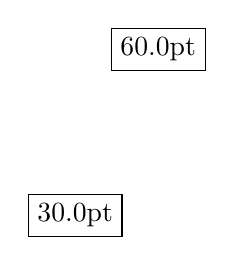
\begin{tikzpicture}[
    x=30pt,
    y=60pt,
  ]
  \SetScales
  \node[draw] at (0,0) { \the\scaledx };
  \node[draw] at (1,1) { \the\scaledy };
\end{tikzpicture}

\end{document}

Anything beyond the document end is a comment, it can be an useful space for
notes.
